\section{Single fluid description of dusty gas}\label{setup} 
We model an accretion disk as a mixture of gas with dust treated as a 
pressureless fluid. We denote their density and
velocity field as $(\rhog,\bm{v}_\mathrm{g})$ and
$(\rhod,\bm{v}_\mathrm{d})$, respectively. The 
mixture has total density \begin{align}
  \rho \equiv \rhog + \rhod,
\end{align}
and center of mass velocity, 
\begin{align}
  \bm{v} \equiv \frac{\rhog\bm{v}_\mathrm{g} + 
    \rhod\bm{v}_\mathrm{d}}{\rho}, 
\end{align}
a single temperature $T$, and its pressure $P$ arise solely from the  
gas component. Our goal is to obtain a set of equations
describing the dust-gas mixture that resembles standard, single-phase
hydrodynamics. 
%This is possible by considering
%strongly coupled dust particles (but not neccessarily perfectly
%coupled) and an isothermal gas equation of state.  

%\subsection{Terminal velocity approximation}

The dust and gas fluids interact via a drag force parameterized by the relative stopping 
time $\tstop$ such that 
\begin{align}  
  \rhod\left.\frac{\p \bm{v}_\mathrm{d}}{\p t}\right|_\mathrm{drag}= -
  \rhog\left.\frac{\p \bm{v}_\mathrm{g}}{\p t}\right|_\mathrm{drag}=
  - \frac{\rhog\rhod}{\rho}\frac{\left(\bm{v}_\mathrm{d} - \bm{v}_\mathrm{g}\right)}{\tstop}. 
\end{align}
is the dust-gas friction force per unit volume. %, where
%\begin{align}
%  \widetilde{\bm{v}} \equiv\bm{v}_\mathrm{d} - \bm{v}_\mathrm{g} 
%\end{align}
%is the dust-gas velocity difference. 
 Note that $\tstop$ 
differs slightly from the \emph{particle} stopping time $\tau_\mathrm{s} =
\tstop\rho/\rhog$ used in some studies
\citep[e.g.][]{youdin05a}. 

In general the relative velocity $\bm{v}_\mathrm{d} -
\bm{v}_\mathrm{g}$ obeys a complicated evolutionary equation 
\citep[see, e.g.][]{youdin05a}. % obtained from taking the difference
%between evolutionary equations for $\bm{v}_\mathrm{g}$ and
%$\bm{v}_\mathrm{d}$. 
 However, for tightly-coupled dust
particles with $\tstop\OmK\ll 1 $, where $\OmK$ is the Keplerian orbital
frequency (since we are interested in protoplanetary disks), we can use the 
`terminal velocity approximation' to set %The dust-gas velocity difference 
%Then so that the dust-gas velocity
%difference is 
\begin{align}
  \bm{v}_\mathrm{d} - \bm{v}_\mathrm{g} = \frac{\nabla
    P}{\rhog}\tstop 
\end{align}
\citep{jacquet11}. This equation reflects the well-known effect of 
particle drift towards pressure maximum  \citep{weidenschilling77}. 

%\subsection{One-fluid equations for dusty gas}

Under the terminal velocity approximation the dust-gas mixture obeys   
the first-order (in $\tstop$) one-fluid equations: 
\begin{align} 
  &\frac{D\rho}{Dt} = -\rho\nabla\cdot\bm{v}, \label{masseq}\\ 
   &\frac{D\tepsilon}{Dt} = -\frac{1}{\rho} \nabla \cdot \left(\tepsilon 
     \tstop \nabla P \right),\label{dusteq}\\
  &\frac{D\bm{v}}{Dt} = - \nabla\Phi_\mathrm{tot} - \frac{1}{\rho}\nabla  P, \label{momeq}\\ 
  &\frac{D T}{D t} = - \left(\gamma-1\right)T\nabla\cdot\bm{v} +
  \mathcal{H} + \mathcal{H}_\mathrm{eff}  - \Lambda  \label{tempeq} 
\end{align} 
\citep[see ][for a detailed derivation from the two-fluid
equations]{laibe14,price15}, where $D/Dt \equiv \p_t +
\bm{v}\cdot\nabla$ is the Lagrangian 
derivative \emph{following the mixture}'s center-of-mass velocity $\bm{v}$. 
For an ideal gas the pressure is given 
by $P = \mathcal{R}\rhog T/\mu $, where $\mathcal{R}$ is
the gas constant and $\mu$ is the mean molecular weight. 



Eq. \ref{dusteq} is obtained from the dust continuity equation,  
$\p_t\rhod + \nabla\cdot\left(\rhod\bm{v}_\mathrm{d}\right)= 0$, 
by writing 
$\bm{v}_\mathrm{d}=\bm{v} + \tstop\nabla P/\rho$, and eliminating  
$\rhod$ in favor of the dust fraction $\tepsilon$: 
\begin{align}
  \tepsilon \equiv \frac{\rhod}{\rho}  = \frac{\epsilon}{1+\epsilon},
\end{align}
where $\epsilon=\rhod/\rhog$ is the usual
dust-to-gas ratio. 
If $\tstop=0$ then the 
dust-to-gas ratio is conserved following the fluid. Otherwise, 
$\epsilon$ evolves due to particle drift in response to pressure
gradients. Note that Eq. \ref{dusteq} is equivalent to Eq. 46 of 
\cite{jacquet11}. 



The total gravitational potential $\Phi_\mathrm{tot}=\Phi +
\psi$ includes that from a central star of mass $M_*$ and the disk's own
potential $\psi$. We adopt 
\begin{align}\label{thin_disk_potential}
  \Phi(r,z) =-\frac{GM_*}{\sqrt{r^2 + z^2}}\simeq
  -\frac{GM_*}{r}\left(1 - \frac{z^2}{2r^2}\right),  
\end{align}
where $(r,\phi, z)$ are cylindrical co-ordinates centered on the star, and 
$G$ is the gravitational constant. The second equality is the  
thin-disk approximation, appropriate for
$|z|\ll r$. We use this approximate form in order to
obtain explicit expressions for disk equilibria (\S\ref{steady_state}). 
The disk potential $\psi$ satisfies the Poisson equation
\begin{align}
  \nabla^2\psi = 4 \pi G \rho.\label{poisson}
\end{align}
We include $\psi$ for
completeness, but we will mostly neglect it unless stated
otherwise.  


For the mixture's temperature evolution, Eq. \ref{tempeq}, 
$\gamma$ is 
the gas adiabatic index; $\mathcal{H}$ represents heating and $\mathcal{H}_\mathrm{eff}$ 
is an effective source term arising from transforming the gas energy equation (Eq. \ref{real_pressure}) 
from the 
two-fluid to one-fluid variables \citep[see][ for 
details]{laibe14}. We also include a simple model of radiative
cooling, 
\begin{align}
  \Lambda = \frac{T -
    T_\mathrm{ref}}{t_\mathrm{cool}}, \label{cooling} 
\end{align}
which relaxes the mixture back to a prescribed temperature profile   
$T_\mathrm{ref}$ on a timescale of $\tcool$. We will shortly simplify
the problem by considering rapid cooling, $\tcool\to0$. 

Eq. \ref{masseq}---\ref{tempeq} are not yet equivalent to standard 
hydrodynamics, which typically evolves two scalar fields: the density and
temperature (or pressure). By contrast, Eq. \ref{masseq}---\ref{tempeq}
involves three scalars: $\rho$, $\tepsilon$, and $T$. 
However, we can establish an  analogy by fixing the gas
equation of state, thus eliminating Eq. \ref{tempeq}; but then reform 
the dust-to-gas ratio evolution equation (\ref{dusteq}) into an
energy-like equation. 

\subsection{Locally isothermal equation of state}\label{loc_iso_eos}
We consider the limit of short cooling 
times, $\tcool\to 0$, appropriate for the outer parts of an irradiated
protoplanetary disk \citep{chiang97,lin15}. Then the disk temperature
$T = T_\mathrm{ref}$ at all times, and so we may
adopt a locally isothermal equation of state 
\begin{align}\label{eos}
  P = c_s^2(r,z)\rhog = c_s^{2}\left(1 - \tepsilon\right)\rho,   
\end{align}
where $c_s(r,z)= \sqrt{\mathcal{R}T_\mathrm{ref}/\mu}$ is a prescribed
sound-speed profile fixed in time. In most applications we consider vertically 
isothermal disks with \begin{align}\label{power_temp}
  c_s^2(r) \propto r^{q},
\end{align}
where $q$ is the power-law index for the disk temperature. For $q=0$
the disk is strictly isothermal.  

Notice Eq. \ref{eos} resembles an ideal gas equation of state but with  
a reduced temperature $\widetilde{T} = 
T_\mathrm{ref}\left(1-\tepsilon\right)$. %sound-speed $c_{s,\mathrm{eff}} = c_s\sqrt{\left(1 -
This reduced temperature decreases with dust-loading. 
%   \tepsilon\right)}$. 
%then the equation of state has the standard
%form $P=c_{s,\mathrm{eff}}^2\rho$. 
Since $\tepsilon$ typically decrease away from the midplane, we expect
vertically isothermal dusty disks to behave as if the temperature
\emph{increased} away from $z=0$.     

\subsection{Effective energy equation}\label{energy_analogy}
Although we have deleted the true energy
equation by fixing a locally isothermal
equation of state, we show that the mixture 
nevertheless obeys an effective energy evolution equation. This is
because advection of the dust-fraction, described by
Eq. \ref{dusteq}, can be transformed into an energy-like 
equation.  
%We show that for a prescribed temperature distribution, the mixture
%obeys an evolutionary energy equation, due to the advection of the
%dust-fraction. 
The equation of state, Eq. \ref{eos}, implies 
\begin{align*}
  \tepsilon = 1 - \frac{P}{c_s^2(r,z)\rho}.  
\end{align*}
Then Eq. \ref{dusteq} becomes
\begin{align}
%\frac{DP}{Dt} 
\frac{\p P}{\p t} + \bm{v}\cdot\nabla P  
&= - P \nabla\cdot\bm{v} + P\bm{v}\cdot\nabla\ln{c_s^2}
                + \mathcal{C},  \label{eff_energy} \\
\mathcal{C}&\equiv c_s^2 \nabla\cdot\left[\tstop\left(1 -
  \frac{P}{c_s^2\rho}\right)\nabla 
  P\right].
\end{align} 
For comparison with the standard energy equation in hydrodynamics,
re-writing Eq. \ref{tempeq} for a pure ideal gas with $P \propto
\rhog T$, and reverting back to gas velocities, gives  
%For later comparison it is convenient to re-write the temperature
%evolution, Eq. \ref{tempeq}, to that for the pressure: 
\begin{align}
  \frac{\p P}{\p t} + \bm{v}_\mathrm{g}\cdot\nabla P = - \gamma P
  \nabla\cdot \bm{v}_\mathrm{g}  +
  \frac{P}{T}\left(\mathcal{H} -
    \Lambda\right).\label{real_pressure} 
%\frac{\rho \mathcal{R}}{\mu}\frac{T
%  - T_\mathrm{ref}}{t_\mathrm{cool}}, \label{realenergy}
\end{align} 
We can thus interpret Eq. \ref{eff_energy} as the energy equation for
and ideal gas with adiabatic index $\gamma=1$, but now with the
imposed temperature gradient $\nabla c_s^2$ and dust-gas drag $\mathcal{C}$ 
acting as source terms. 

%playing the
%role of radiative cooling ($\Lambda$ in 
%Eq. \ref{tempeq}). 
%In this form, the function $\mathcal{C}$ can be interpreted
%as a cooling term. 
   
If we denote 
\begin{align}
  \bm{F} \equiv  - \frac{\nabla P}{\rho}
\end{align}
for the pressure forces, then
\begin{align*}
  \mathcal{C} = - c_s^2\nabla \left( \tepsilon \tstop \rho \bm{F}
  \right), 
\end{align*}
which is in the same form as cooling by radiative diffusion. In protoplanetary
disks the corresponding `heat flux', proportional to $\bm{F}$, is
directly radially outwards and vertically upwards. This is simply a
reflection of particle drift towards increasing pressure (inwards and 
downwards). Particle flux into a region contributes to `cooling' of
that region because the reduced temperature is lowered. 

% Eq. \ref{eff_energy} can be written in conservative form,
% \begin{align*}
%   \frac{\p P}{ \p t} + \nabla\cdot\left\{P\left[\bm{v} -
%       \tstop\left(c_s^2 - \frac{P}{\rho}\right)\nabla\ln{P}\right]
%     \right\}\\
%   = \left[P\bm{v} - \tstop\left(c_s^2 - \frac{P}{\rho}\right)\nabla
%     P\right]\cdot\nabla\ln{c_s^2}. 
% \end{align*} 
% We may thus re-interpret $P$ as the mixture's energy density, but the
% energy flux has an additional contribution from the pressure
% gradient and dust-gas friction. The term on the right-hand-side, owing
% to the imposed temperature profile, can be interpreted as an external
% heat source.  

%We comment that 

%An effective energy equation can also be derived for other 
%fixed gas equations of state, such as polytropic gas. We discuss this
%in \S\ref{gen_poly}.

\subsection{Entropy and buoyancy of isothermal dusty gas }\label{dusty_entropy}

The specific entropy of an ideal gas is 
$S~=~C_P\ln{\left(P^{1/\gamma}/\rhog\right)}$, where $C_P$ is the heat 
capacity at constant pressure. 

Since we have shown that a locally isothermal dusty gas effectively
has $\gamma=1$ we can define an effective 
entropy for the \emph{mixture} as 
\begin{align}
   \seff \equiv \ln \frac{P}{\rho} = \ln{\left[c_s^2(1-\tepsilon)\right]},  
\end{align} 
where the constant heat capacity has been absorbed into $\seff$. 
%This follows naturally by combining the effective 
%energy Eq. \ref{eff_energy} and Eq. \ref{masseq}. 
Then combining Eq. \ref{eff_energy} and \ref{masseq} gives  
\begin{align*}
  \frac{D \seff}{D t} = \bm{v}\cdot\nabla\ln{c_s^2} +
  \frac{c_s^2}{P}\nabla\cdot\left(\tstop\tepsilon\nabla P\right), 
\end{align*}
which is equivalent to entropy evolution in standard  
hydrodynamics, albeit with source terms. With an effective
entropy defined this way, many of the  
results concerning the stability of (locally) isothermal dusty gas
will have identical form and interpretations to that for pure gas.   

%If $c_s^2$ is constant and $\tstop=0$, then 
%$D\seff/ D t = D\tepsilon/D t=0$. In this case the effective 
%entropy is conserved because the dust-fraction is `frozen in' the
%flow. 

The physical reason for this analogy is that with strong drag
($\tstop\to0$), dust is almost perfectly entrained in the gas, but
there is some gain/loss of dust particles between different  
gas parcels. This is analogous to the entropy of an ideal 
pure gas subject to heating/cooling: entropy is conserved following
a gas parcel, except if there is heat exchange between a fluid parcel and the
surrounding. For strictly isothermal gas perfectly coupled to dust
(constant $c_s^2$ and $\tstop=0$) we have 
$D\seff/ D t = D\tepsilon/D t=0$. In this case the effective 
entropy is exactly conserved because the dust-fraction is `frozen in' the
flow. 


%\subsection{Dusty buoyancy forces}
We can now define the vertical buoyancy frequency $N_z$ of the mixture
as    
%$N_z$ of the mixture is given by 
\begin{align}
  N_z^2 \equiv - \frac{1}{\rho}\frac{\p P}{\p z}\frac{\p \seff}{\p z}
  =c_s^2(r) \frac{\p \ln{\rhog}}{\p z}\frac{\p \tepsilon}{\p z},
%  \quad 
 % N_z^2 \equiv - \frac{1}{\rho}\frac{\p P}{\p z}\frac{\p \seff}{\p z}.
%&=
  %\frac{c_s^2(r)}{\left(1+\epsilon\right)^2}\frac{\p\ln\rhog}{\p 
%  z}\frac{\p\epsilon}{\p z} \\ &
  %                                =
 % \frac{\epsilon}{\left(1+\epsilon\right)^2}\left(\frac{z}{\Htilde}\right)^2\OmK^2\notag,  
\end{align}
%Typically in a thin, smooth disk we have $|N_r|\ll |N_z|$. 
where the second equality assumes a vertically isothermal disk. 
Protoplanetary disks have $\p_z\rhog<0$, thus stability against vertical 
convection ($N_z^2>0$) requires $\p_z\tepsilon <0 $, i.e. the dust density should drop faster 
than the gas density away from the midplane. 
This is equivalent to 
entropy increasing away from the midplane. A similar expression exists
for the radial buoyancy frequency $N_r$, but $|N_r|\ll |N_z|$ in thin,
smooth disks. 

A vertical buoyancy force exists even in vertically isothermal
dusty disks, because coupling gas to dust particles increases
the fluid's inertia, but pressure (i.e. restoring) forces are
unchanged. The increased weight of the fluid resists vertical
oscillations and hence there is an associated buoyancy force. However,
if $\tstop\neq0$ so the gas-dust coupling is imperfect, then gas is no
longer `weighed down' by the dust, and can slip past it. Thus finite
drag diminishes the dust-induced buoyancy. This is similar to reducing
gas buoyancy through cooling \citep{lin15}. 

%{\bf
\subsection{Physical disk conditions}
%physical disk conditions underwhich the above approx
%(small/well-coupled dust and isothermal gas) is applicable. smaller
%than mm at few tens of au. give dimensional numbers here
%}
The above correspondence between isothermal dusty gas and adiabatic
pure gas is derived under the terminal velocity approximation, which applies
to short stopping times, $\tstop\OmK\ll 1$; and the locally isothermal
approximation, which applies to short cooling times, $t_\mathrm{cool}\OmK\ll
1$. In typical protoplanetary disk
models such as the Minimum Mass Solar Nebula, $\tstop$ decreases for
smaller particles and/or towards smaller radii \citep{youdin11}. However,
$t_\mathrm{cool}$ is generally only small in the outer disk
\citep{lin15,malygin17}. Combining these results, we estimate the 
correspondence will be applicable to particles less than mm in size at a few
to 10s of AU in protoplanetary disks. However, note that the
isothermal approximation may be relaxed to other fixed equations of
state (see \S\ref{gen_poly}). 


\section{General stability criteria for dusty gas}\label{limits}

In this section we discuss the stability properties of the 
dusty-gas mixture using a variational principle. This approach does not
require explicit solutions (i.e. a specific distribution of the density and dust-to-gas ratio)  
to the equilibrium equations. We consider axisymmetric systems and neglect self-gravity here.  

\subsection{Steady states}\label{eqm}
%We consider axisymmetric steady states as background equilibria to
%perturb. 

For a given distribution of the dust-fraction $\tepsilon$ (or
dust-to-gas ratio $\epsilon$), the 
mass and momentum Eqs. \ref{masseq}---\ref{momeq} admit     
solutions with $\rho(r,z)$ and 
$\bm{v}=r\Omega(r,z)\hat{\bm{\phi}}$ where $\Omega = v_\phi/r$, which satisfy 
\begin{align}
  r\Omega^2 &= \frac{\p \Phi}{\p r} + \frac{1}{\rho}\frac{\p P}{\p
    r},\label{steady_momr}\\
  0 & = \frac{\p\Phi}{\p z} + \frac{1}{\rho}\frac{\p P}{\p z},\label{steady_momz}
%  0 & = \nabla\cdot\left(\tepsilon\tstop\nabla P\right) \label{steady_dust}
\end{align}
with $P=P(\tepsilon,\rho)$ given by the equation of state
(Eq. \ref{eos}). An explicit solution is presented in 
\S\ref{steady_state}, when we analyze the stability of
protoplanetary disks. 

The mixture possess vertical shear. To see this, we eliminate $\Phi$
between Eq. \ref{steady_momr}---\ref{steady_momz} to 
obtain 
\begin{align}\label{vshear}
  r\frac{\p \Omega^2}{\p z} 
%&= \frac{\p\ln{\rho}}{\p r}\frac{\p}{\p
%    z}\left[c_s^2(1-\tepsilon)\right] - \frac{\p\ln{\rho}}{\p z}
%  \frac{\p}{\p r} \left[c_s^2(1-\tepsilon)\right]\\  
   &= \frac{1}{\rho}\left(\frac{\p P}{\p r}\frac{\p \seff}{\p z} -\frac{\p
    P}{\p z}\frac{\p \seff}{\p r} \right).% \\
%& = \frac{1}{\rhog}\left(\frac{\p P}{\p r}\frac{\p \seff}{\p z} -\frac{\p
%    P}{\p z}\frac{\p \seff}{\p r} \right)
\end{align}
and recall $\seff = \ln{\left[c_s^2\left(1-\tepsilon\right)\right]}$. It is well appreciated that 
vertical stratification of the dust layer contributes to vertical shear
\citep{chiang08}. Eq. \ref{vshear} shows that a radial dust
stratification ($\p_r\tepsilon$) also contributes to vertical shear.  

%Since $\seff$ depends on $\tepsilon$, we see that radial gradients in
%the dust-to-gas ratio also drives vertical shear \citep[cf. that 
%driven by $\p_z\epsilon$ usually discussed in dusty disks,  
%e.g.][]{chiang08}. 


Our equilibrium solutions satisfy the hydrostatic constraints of
Eq. \ref{steady_momr}---\ref{steady_momz} but are not in general
steady state solutions to the energy 
equation (\ref{eff_energy}), because the source term $\mathcal{C} \ne0$ for realistic disks.  
Limiting cases with $\mathcal{C} \equiv 0$ include \begin{inparaenum}[1)] 
\item 
  unstratified or 2D, razor-thin disk models with finite dust-gas drag; %(\S\ref{si});   
\item 
  perfectly-coupled dust with $\tstop=0$. %(\S\ref{results}). 
\end{inparaenum} 
The following analyses thus apply strictly to these limiting cases of
$\mathcal{C} = 0$ in equilibrium.  Our analysis is also a good approximation when 
$\tstop$ is sufficiently small such that the evolution of the background disk (e.g. dust-settling) 
occur on much longer timescales than the instability growth timescales. 



%However, disk structures obtained from
%Eq. \ref{steady_momr}---\ref{steady_momz} generally do not satisfy  
%the steady state effective energy Eq. \ref{eff_energy} because typically 
%$\mathcal{C}\neq0$.  In order to have a well-defined stability problem, we formally
%consider equilibria with $\mathcal{C}\equiv 0$. Namely      
%\begin{inparaenum}[1)] 
%\item 
%  unstratified or 2D disks with finite dust-gas drag; %(\S\ref{si});   
%\item 
%  perfectly-coupled dust with $\tstop=0$. %(\S\ref{results}). 
%\end{inparaenum} 
%Alternatively, we are assuming that $\tstop$  is sufficiently small





 % N_z^2 
%\end{align}

%\section{Limiting behaviours}\label{limits}


\subsection{Integral relation}

%Our discussion is based on
%the corresponding axisymmetric linearized equations. 
We consider axisymmetric Eulerian perturbations to a variable $X$ of
the form  
\begin{align}
 \real\left[ \delta X(r,z)\exp{\left(-\ii\sigma t\right)}\right], 
\end{align}
where $\sigma$ is the complex mode frequency. We 
write 
\begin{align}
  \sigma = \ii s - \omega,
\end{align}
where $s$ and $\omega$ are the growth rate and real frequencies,
respectively. Then perturbations have time dependence $e^{st +
  \ii\omega t}$.  Thus for $\omega>0$, perturbations rotate
anti-clockwise in the complex plane. 

In Appendix \ref{var_prin} we linearize Eqs. \ref{masseq}, \ref{momeq}, and 
Eq. \ref{eff_energy} to derive the following integral relation: 
\begin{align}
%&  \sigma^2\int\rho\left(|\dd v_r|^2 + |\dd v_z|^2\right)dV \notag\\
  \sigma^2\mathcal{I}^2
&= \int\left[ \rho
  |\dd v_r|^2A + \rho  \left(\dd v_z \dd v_r^* + \dd v_z^*\dd v_r\right) B +
  \rho |\dd v_z|^2 D\phantom{\frac{1}{1}}\right. \notag\\
&\phantom{===}  \left. + \frac{1}{P}\Bigl\lvert \nabla\cdot\left(P\dd
  \bm{v}\right)\Bigr\rvert^2\right]dV  -\int \left(\nabla\cdot\dd\bm{v}^*\right)\dd\mathcal{C}dV \notag\\
&\phantom{===}
- \int P
  \left(\nabla\cdot\dd\bm{v}^*\right)\left(\dd\bm{v}\cdot\nabla\ln{c_s^2}\right)dV,\label{int_rel}
\end{align} 
%The real integral $\mathcal{I}^2>0$ 
where $^*$ denotes the complex conjugate, 
\begin{align}
  \mathcal{I}^2 \equiv \int\rho\left(|\dd v_r|^2 + |\dd v_z|^2\right)dV
\end{align}
is the meridional kinetic energy, 
and coefficients $A,B,D$ can be 
read off Eq. \ref{integral_ex}. %Note that $B=C$ from dynamical equilibrium
%(Eq. \ref{vshear}). 
We now consider various limits of Eq. \ref{int_rel}.    


\subsection{Strictly isothermal gas perfectly coupled to dust}\label{iso_perfect}
When $c_s^2$ is a constant and $\tstop=0$ (so that $\mathcal{C} = 0$), the dusty-gas equations are
exactly equivalent to that for adiabatic hydrodynamics with unit
adiabatic 
index. Although the gas is strictly isothermal, the mixture behaves 
adiabatically because the dust fraction $\tepsilon$ is advected with 
the gas. This is similar to entropy conservation following an 
adiabatic gas without heating or cooling.  

In this case, the last two integrals in Eq. \ref{int_rel} vanish. 
Then the condition for axisymmtric \emph{stability}, $\sigma^2>0$, 
is met if the integrand coefficients satisfy $A+D>0$ and $AD-B^2>0$
\citep[][Section 11.6]{ogilvie16}, which becomes 
\begin{align}
  \kappa^2 + \frac{1}{\rhog}\nabla P \cdot\nabla\tepsilon &> 0,\label{dusty_solberg1}  \\
  -\frac{1}{\rhog}\frac{\p P}{\p z}\left(-\kappa^2\frac{\p\tepsilon}{\p
    z} + r\frac{\p\Omega^2}{\p z}\frac{\p \tepsilon}{\p r} \right) & > 0, \label{dusty_solberg2}
\end{align} 
%\begin{align}
%  \kappa^2 + c_s^2 \nabla\ln{\rhog}\cdot\nabla\tepsilon &> 0,\label{dusty_solberg1}  \\
%  -c_s^2\frac{\p\ln{\rhog}}{\p z}\left(-\kappa^2\frac{\p\tepsilon}{\p
%    z} + r\frac{\p\Omega^2}{\p z}\frac{\p \tepsilon}{\p r} \right) & > 0, \label{dusty_solberg2}
%\end{align} 
%\begin{align}
%  \kappa^2 - \frac{1}{\rho}\nabla P \cdot \nabla s &> 0, \label{dusty_solberg1}    \\
%  -\frac{1}{\rho}\frac{\p P}{\p z} \left(\kappa^2 \frac{\p s}{\p z} -
%  r\frac{\p\Omega^2}{\p z}\frac{\p s}{\p r}\right) &>0, \label{dusty_solberg2}
%\end{align} 
where %$s = \ln{P/\rho}$, 
$\kappa^2 \equiv r^{-3}\p_r\left(r^4\Omega^2\right)>0$ is the 
square of the epicylic frequency. Note that $\nabla P/\rhog =
c_s^2\nabla \ln{\rhog}$ for strictly isothermal gas considered here. 
 
Eq. \ref{dusty_solberg1}---\ref{dusty_solberg2} can in fact be obtained by
inserting $C_P\ln{\left(1 - 
    \tepsilon\right)}$ for the entropy into the standard
expression for the Solberg-Hoiland criteria 
\citep{tassoul78} for axisymmetric stability of adiabatic gas. 
This substitution is 
consistent with our definition of the effective entropy $\seff$ since
we are considering constant $c_s$. 

We expect Eq. \ref{dusty_solberg1} to be satisfied in typical
protoplanetary disks where the dust-to-gas ratio increases in the same
direction as the local pressure gradient, which is equivalent to the
gas density gradient for isothermal gas. 

On the other hand, Eq. \ref{dusty_solberg2} can be violated in
disks if the dust is vertically well-mixed but radially-stratified,  
such that $\p_z\tepsilon = 0$ but $\p_r\tepsilon\neq0$. In this case the
left-hand-side of Eq. \ref{dusty_solberg2} becomes
\begin{align}
-\left(\frac{1}{\rhog}\frac{\p P}{\p
    z}\right)^2\left(\frac{\p\tepsilon}{\p r}\right)^2<0.
\end{align}
%\begin{align}
%-c_s^4\left(\frac{\p\ln{\rhog}}{\p
%    z}\right)^2\left(\frac{\p\tepsilon}{\p r}\right)^2<0.
%\end{align}
Such an isothermal dusty disk is \emph{unstable} because there is no
effective vertical buoyancy to stabilize vertical motions ($N_z=0$),
which can tap into the free energy associated with  
vertical shear due to the radial gradient in the dust-fraction. 
This situation is identical to the pure gas, adiabatic simulations of \cite{nelson13}
where the gas entropy is vertically uniform but has a radial
gradient. The authors indeed find instability. We give a numerical
example in the dusty context in \S\ref{vert_mixed}.   

\subsection{Thermodynamics of dust-drag instabilities}\label{dust_work}
The physical interpretation of \S\ref{grow_osc} is here derived in
detail. Consider constant $c_s$ but $\tstop\neq0$ (so $\delta\mathcal{C}
\neq 0$). Eq. \ref{int_rel} indicates that $\sigma^2$ is generally complex, so
we may have growing oscillations, or overstability, due to dust-gas
friction. This is seen by taking the imaginary part of
Eq. \ref{int_rel} 
\begin{align}
%  s = \frac{\imag\int \left(\nabla\cdot\dd\bm{v}^*\right)\dd\mathcal{C}dV}{2\omega\int\rho\left(|\dd
%    v_r|^2 + |\dd v_z|^2\right)dV}, \label{thermal_instability}
  s = \frac{\imag\int \left(\nabla\cdot\dd\bm{v}^*\right)\dd\mathcal{C}dV}{2\omega\mathcal{I}^2}, \label{thermal_instability}
\end{align} 
assuming $\omega\neq0$. %This represents overstability due to dust-gas friction. 
Since drag ($\delta \mathcal{C}$) appears as a source term in our
effective energy equation, the quantity 
$\imag\left[\left(\nabla\cdot\dd\bm{v}^*\right)\dd\mathcal{C}\right]$
represent correlations between compression/expansion and  
heating/cooling.  

It is well-known that such correlations may lead to pulsational
instabilities in stars \citep{cox67}. We thus interpret  
dust-drag overstabilities in a similar way, 
adapting from the treatment of stellar 
pulsations by \cite{cox67} and lecture notes by \cite{samadi15} and 
J. Christensen-Dalsgaard\footnote{\url{http://astro.phys.au.dk/$\sim$jcd/oscilnotes/print-chap-full.pdf}}.        
 
%and disks
%\cite{kato78}. 


\subsubsection{Work done by dusty gas} 

The physical interpretation of Eq. \ref{thermal_instability} is that 
work done by pressure forces in the dusty gas leads to growth in
oscillation amplitudes. To demonstrate this, we calculate the average
work done assuming periodic oscillations, and show that if the average
work done is positive, then the 
oscillation amplitude would actually grow. 

Consider oscillations in the dusty gas with period $T_p$. 
The average rate of work done is 
\begin{align}
  \mathcal{W} = \frac{1}{T_p}\int^{t+T_p}_{t}dt^\prime\int_M P
  \frac{D\upsilon}{Dt^\prime} dm \label{work_def} 
\end{align}
\citep[][see their Eq. 4.10 and related discussions]{cox67}, 
where $\upsilon=1/\rho$ is the specific volume of the mixture, $D/Dt$
is the Lagrangian derivative, and the 
spatial integral is taken over the total mass $M$ of the mixture and
$dm$ is a mass element. 

Noting that only products of perturbations contribute to
$\mathcal{W}$, we find that for periodic oscillations (time dependence 
$e^{\ii\omega t}$ and real $\omega$): 
\begin{align}
  \mathcal{W} = - \frac{\omega}{2} \int \imag\left(\Delta P
  \frac{\Delta \rho^*}{\rho}\right)dV,\label{work_real}
\end{align}
where %the integral is taken over the volume of the
%mixture; and 
 the Lagrangian perturbation $\Delta$ of a variable $X$ is 
$\Delta X = \delta X + \bm{\xi}\cdot\nabla X$ 
and $\bm{\xi}$ is the
Lagrangian displacement ($    \xi_{x,z} =  \ii \dd v_{x,z}/\sigma$).  
Eq. \ref{work_real} show that a phase difference between gas pressure and
the total density leads to work done
($\mathcal{W}\neq0$).  

Now, Eq. \ref{lin_mass_full}---\ref{lin_energy_full} 
imply the integrand of the numerator in Eq. \ref{thermal_instability} 
is 
\begin{align} 
  \imag \left(\delta \mathcal{C}
  \nabla\cdot\dd \bm{v}^*\right) = 
  -|\sigma|^2\imag \left(\Delta P 
  \frac{\Delta\rho^*}{\rho}\right), \label{pdv}
\end{align}
for constant $c_s$. 
%This states that `PdV' work (the right-hand-side) is 
%provided by dust-drag friction, and can be seen explicitly as 
%follows. 
Then combining Eq. \ref{work_real}, \ref{pdv} and
\ref{thermal_instability} 
gives  
\begin{align}
s = \frac{\mathcal{W}}{\mathcal{I}^2}, \label{growth_work}
\end{align}
where we have set $\sigma= - \omega$ in 
Eq. \ref{pdv}. Eq. \ref{growth_work} states that if the average work
done is positive during an oscillation, $\mathcal{W}>0$, 
then its amplitude would actually grow ($s>0$).  %and not be periodic 

Positive work is done by a fluid parcel if $-\omega \imag\left(\Delta  
P\Delta\rho^*\right)>0$. Without loss of generality, take $\omega>0$
and consider a mass element with $\Delta\rho = 1$. Then positive work 
requires $\imag\left(\Delta
P\right)<0$.  This corresponds to Lagrangian pressure perturbations \emph{lagging}
behind that in density, see Fig. \ref{lag_cartoon}
for the case of dusty gas.   

%, since the phase of
%the assumed perturbations increase in time.  
%$\imag\left(\Delta\rho\right)=0$.   


\begin{figure}
  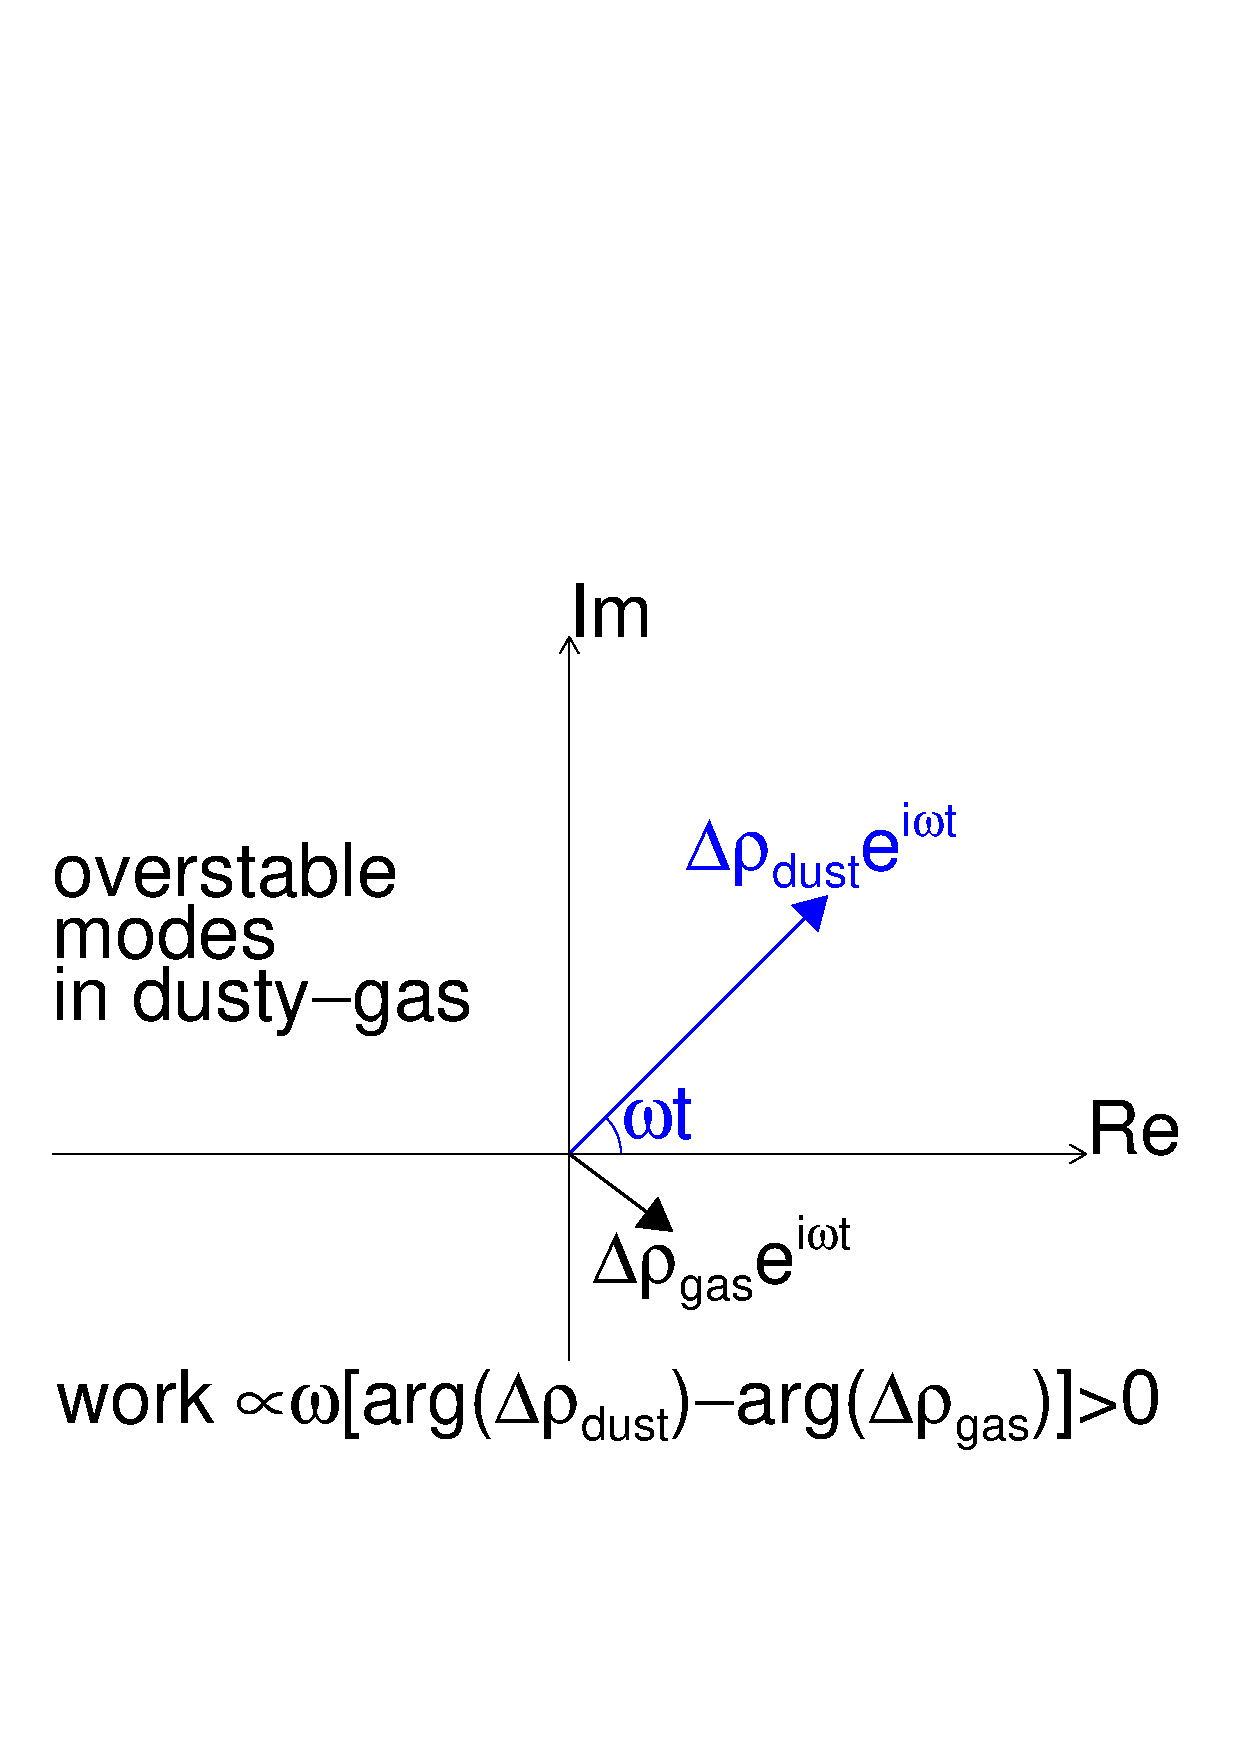
\includegraphics[width=\linewidth,clip=true,trim=0cm 5cm 0cm 0cm]{figures/lag}
  \caption{Phase relation for overstable modes in isothermal dusty
    gas. Such modes require (Lagrangian) oscillations in the gas
    pressure, which is directly proportional to the gas density, to
    lag behind that in dust density. The eigenvectors rotate anti-clockwise for $\omega>0$. 
    \label{lag_cartoon}
  }
\end{figure}


\subsubsection{Physical property of dust-gas drag overstabilities}  

%We now use physical arguments to show that $\mathcal{W}>0$ if pressure
%perturbations (from the gas) lags behind the total density of the gas
%plus dust mixture. 
%The full energy equation is  
%\begin{align*}
%  \frac{DP}{Dt} = \frac{P}{\rho}\frac{D\rho}{D t} + \mathcal{C}. 
%\end{align*} 
%Dust-drag causes a phase difference between the pressure and density 
%evolution of a fluid element. 

%Consider a fluid element at maximum density during an
%oscillation cycle (point $A$), so that $D\rho/ D t = 0$. If dust-gas
%drag provides an effective heating to the fluid element at $A$
%(i.e. gas influx)  then it will experience increasing pressure, $DP/D
%t>0$. It attains pressure maximum (point $B$) \emph{after} reaching
%density maximum. 

%Applying the above argument to isothermal dusty gas, 

The above discussion applies to any single fluid with a pressure and
density. In the case of interest --- dusty gas --- the work done 
is attributed to finite dust-gas drag. 
%For dusty gas, the work done during oscillations 
 %is attributed to finite dust-gas drag. 
The relative 
drift between gas and dust causes a phase difference between the two
components, and hence between pressure and total density. 

A parcel of the strictly isothermal dusty-gas mixture does 
positive work if  
\begin{align*}
-\sgn\left(\omega\right)\imag\left(\Delta\rhog\Delta\rhod^*\right)>0,
\end{align*}
meaning that gas follows dust (Fig. \ref{lag_cartoon}). Overstabilities 
are thus not possible if the gas does not respond to dust 
(i.e. no back-reaction).% {\bf can we say this means that any effective
%  dust-drag instability require high dust to gas ratios?} 
The pressure-density lag shown in
Fig. \ref{lag_cartoon} is achieved if, just after the total density of a 
parcel maximizes, its gas content
is increasing, which requires a sufficiently large
particle flux \emph{out} of the parcel. See $A$ to $B$ in 
Fig. \ref{pdv_cartoon}. 

%{\bf lagrangian derivative follows the mixture.}
% this highlights one
%  perk of the one-fluid framework. in two-fluid models there are two
%  types of lagragian deriv, not clear which fluid to follow.}

This thermodynamic interpretation does not explain 
why drag forces causes gas pressure to lag behind the dust
density, but shows 
that this \emph{must} be the case for any growing oscillations associated the
dust-gas drag. To rigorously understand how dust-drag causes this 
lag requires an explicit solution to the linearized equations with 
detailed treatment of the function $\mathcal{C}$. However, given the complexity of
$\mathcal{C}$ (see Appendix \ref{lin_dust}), we might generally expect
 dusty disks to  support a range of stable and overstable modes, with the
latter being associated with pressure-density lag. 
%Indeed, \cite{jacquet11} explains the essence of the streaming 
%instability in dusty protoplanetary disks as dust accumulation
%(and hence compression) at a pressure bump, which then drags the 
%gas towards it (and hence heating) to strengthen the pressure
%bump. That is, heating occurs upon compression, as in stellar  
%pulsational instabilities \citep{cox67}.
 In \S\ref{si} we check that the
streaming instability fits into this thermodynamic interpretation in
the strong drag limit.  




%A phase difference was also noted in the 
%numerical calculations of the streaming instability by 
%\citet{youdin07b}.    

%Whether the phase
%difference is positive or negative depends on the cooling function
%$\mathcal{C}$, but we may expect a system to generally have both
%modes, and that with a phase lag are unstable. 

\subsection{Locally isothermal gas perfectly coupled to dust}\label{dusty_vsi_int}
If $c_s(r,z)$ is non-uniform but $\tstop=0$, Eq. \ref{int_rel} 
gives  
\begin{align}
%  s = \frac{\imag\int P
%  \left(\nabla\cdot\dd\bm{v}^*\right)\left(\dd\bm{v}\cdot\nabla\ln{c_s^2}\right)dV}{2\omega\int\rho\left(|\dd 
%    v_r|^2 + |\dd v_z|^2\right)dV}. \label{vsi_check} 
  s = \frac{\imag\int P
    \left(\nabla\cdot\dd\bm{v}^*\right)\left(\dd\bm{v}\cdot\nabla\ln{c_s^2}\right)dV}{2\omega\mathcal{I}^2}, \label{vsi_check} 
\end{align} 
again assuming $\omega\neq0$. 
This instability represents VSI caused by vertical shear arising from a radial
temperature gradient \citep{nelson13,barker15,lin15}. We present 
numerical solutions of the VSI with perfectly-coupled dust in \S\ref{results}. 
